% This file was created with tikzplotlib v0.10.1.
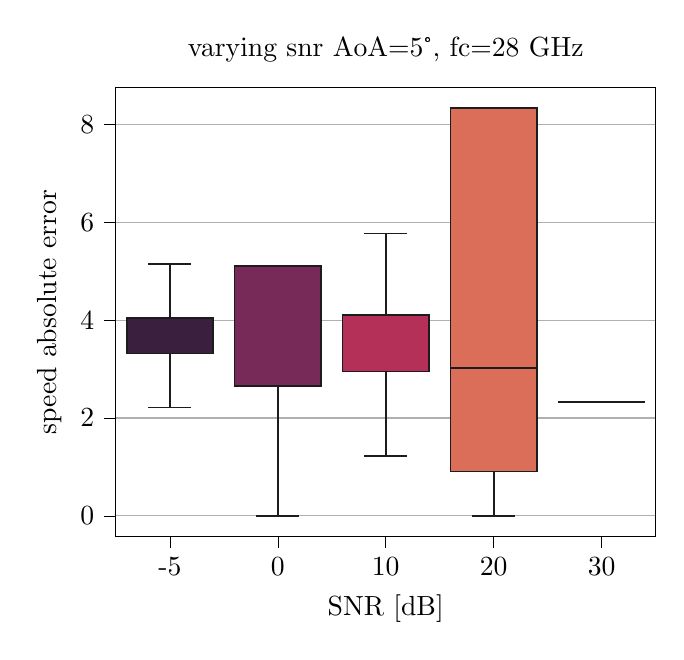
\begin{tikzpicture}

\definecolor{black28}{RGB}{28,28,28}
\definecolor{brown1814888}{RGB}{181,48,88}
\definecolor{burlywood231175145}{RGB}{231,175,145}
\definecolor{darkgray176}{RGB}{176,176,176}
\definecolor{darkslategray583162}{RGB}{58,31,62}
\definecolor{indianred21811088}{RGB}{218,110,88}
\definecolor{purple1194288}{RGB}{119,42,88}

\begin{axis}[
tick align=outside,
tick pos=left,
title={varying snr AoA=5°, fc=28 GHz},
x grid style={darkgray176},
xlabel={SNR [dB]},
xmin=-0.5, xmax=4.5,
xtick style={color=black},
xtick={0,1,2,3,4},
xticklabels={-5,0,10,20,30},
y grid style={darkgray176},
ylabel={speed absolute error},
ymajorgrids,
ymin=-0.41641801724675, ymax=8.75211339788454,
ytick style={color=black}
]
\path [draw=black28, fill=darkslategray583162, semithick]
(axis cs:-0.4,3.31707627403857)
--(axis cs:0.4,3.31707627403857)
--(axis cs:0.4,4.04965417726733)
--(axis cs:-0.4,4.04965417726733)
--(axis cs:-0.4,3.31707627403857)
--cycle;
\path [draw=black28, fill=purple1194288, semithick]
(axis cs:0.6,2.65901380003984)
--(axis cs:1.4,2.65901380003984)
--(axis cs:1.4,5.10355959993171)
--(axis cs:0.6,5.10355959993171)
--(axis cs:0.6,2.65901380003984)
--cycle;
\path [draw=black28, fill=brown1814888, semithick]
(axis cs:1.6,2.95463019224071)
--(axis cs:2.4,2.95463019224071)
--(axis cs:2.4,4.11024710836443)
--(axis cs:1.6,4.11024710836443)
--(axis cs:1.6,2.95463019224071)
--cycle;
\path [draw=black28, fill=indianred21811088, semithick]
(axis cs:2.6,0.905278060732711)
--(axis cs:3.4,0.905278060732711)
--(axis cs:3.4,8.33536148023216)
--(axis cs:2.6,8.33536148023216)
--(axis cs:2.6,0.905278060732711)
--cycle;
\path [draw=black28, fill=burlywood231175145, semithick]
(axis cs:3.6,2.32415810579255)
--(axis cs:4.4,2.32415810579255)
--(axis cs:4.4,2.32415812328389)
--(axis cs:3.6,2.32415812328389)
--(axis cs:3.6,2.32415810579255)
--cycle;
\addplot [semithick, black28]
table {%
0 3.31707627403857
0 2.2187410845062
};
\addplot [semithick, black28]
table {%
0 4.04965417726733
0 5.14762831612689
};
\addplot [semithick, black28]
table {%
-0.2 2.2187410845062
0.2 2.2187410845062
};
\addplot [semithick, black28]
table {%
-0.2 5.14762831612689
0.2 5.14762831612689
};
\addplot [semithick, black28]
table {%
1 2.65901380003984
1 0.000544246747101518
};
\addplot [semithick, black28]
table {%
1 5.10355959993171
1 5.1035595999319
};
\addplot [semithick, black28]
table {%
0.8 0.000544246747101518
1.2 0.000544246747101518
};
\addplot [semithick, black28]
table {%
0.8 5.1035595999319
1.2 5.1035595999319
};
\addplot [semithick, black28]
table {%
2 2.95463019224071
2 1.22259624659547
};
\addplot [semithick, black28]
table {%
2 4.11024710836443
2 5.77063824949806
};
\addplot [semithick, black28]
table {%
1.8 1.22259624659547
2.2 1.22259624659547
};
\addplot [semithick, black28]
table {%
1.8 5.77063824949806
2.2 5.77063824949806
};
\addplot [semithick, black28]
table {%
3 0.905278060732711
3 0.000333410713763582
};
\addplot [semithick, black28]
table {%
3 8.33536148023216
3 8.33536196992403
};
\addplot [semithick, black28]
table {%
2.8 0.000333410713763582
3.2 0.000333410713763582
};
\addplot [semithick, black28]
table {%
2.8 8.33536196992403
3.2 8.33536196992403
};
\addplot [semithick, black28]
table {%
4 2.32415810579255
4 2.32415807966589
};
\addplot [semithick, black28]
table {%
4 2.32415812328389
4 2.32415812328389
};
\addplot [semithick, black28]
table {%
3.8 2.32415807966589
4.2 2.32415807966589
};
\addplot [semithick, black28]
table {%
3.8 2.32415812328389
4.2 2.32415812328389
};
\addplot [semithick, black28]
table {%
-0.4 4.04965417687992
0.4 4.04965417687992
};
\addplot [semithick, black28]
table {%
0.6 5.10355955583013
1.4 5.10355955583013
};
\addplot [semithick, black28]
table {%
1.6 4.11024710768552
2.4 4.11024710768552
};
\addplot [semithick, black28]
table {%
2.6 3.01697378881273
3.4 3.01697378881273
};
\addplot [semithick, black28]
table {%
3.6 2.32415812328362
4.4 2.32415812328362
};
\end{axis}

\end{tikzpicture}
